\documentclass{standalone}
\usepackage{tikz}
\usepackage{ctex,siunitx,ninecolors}
\setCJKmainfont{Noto Serif CJK SC}
\usepackage{tkz-euclide}
\usepackage{amsmath}
\usepackage{wasysym}
\usetikzlibrary{patterns, calc}
\usetikzlibrary{decorations.pathmorphing, decorations.pathreplacing, decorations.shapes,3d}
\newcommand\dlj[2][0]{
  \begin{scope}[#2,scale=1.8]
    \begin{scope}[z={(-10:10mm)},x={(30:10mm)}]
      \begin{scope}[canvas is yz plane at x=-0.25]
        \draw[fill=lightgray](0,-0.5)rectangle(-0.1,0.5);
      \end{scope}
      \begin{scope}[canvas is xy plane at z=0.5]
        \draw[fill=darkgray](0.25,-0.1)rectangle(-0.25,0);
      \end{scope}
      \begin{scope}[canvas is zx plane at y=0]
        \draw[fill=gray](-0.5,-0.25)rectangle(0.5,0.25);
      \end{scope}
      \begin{scope}[canvas is yz plane at x=-0.2]
        \draw[fill=lightgray!50](0,-0.4)rectangle(1.2,0.4);
        \foreach \x in {-30,-20,...,20}
        {
          \draw[ultra thin] ([shift=(\x:0.6)]0.4,0)--++(\x:-0.1);
          \draw[ultra thin] ([shift=(\x+5:0.6)]0.4,0)--++(\x+5:-0.08);
          \foreach \y in {1,2,3,4,6,7,8,9}
          {
            \draw[ultra thin] ([shift=(\x+\y:0.6)]0.4,0)--++(\x+\y:-0.05);
          }
        }
        \draw[ultra thin] ([shift=(30:0.6)]0.4,0)--++(30:-0.1);
        \draw[very thin,red] (0.4,0)--++(#1:0.65)(0.4,0)--++(#1:-0.05);
        \draw[fill=gray](0.4,0)circle(0.02);
        \draw[very thin,fill=darkgray](0.3,-0.1)--++(0.15,0)arc(-90:90:0.1)--(0.3,0.1)--(0.3,0.05)--++(0.15,0)arc(90:-90:0.05)--(0.3,-0.05)--cycle;
        \draw[fill=cyan!20,fill opacity=0.5,very thin](0.3,-0.35)rectangle(1.1,0.35);
        \coordinate (in) at (0.2,0.25);
        \coordinate (out) at (0.2,-0.25);
        \fill[darkgray](in)circle(0.8pt)(out)circle(0.8pt);
      \end{scope}
      \begin{scope}[canvas is xy plane at z=0.4]
        \draw[fill=darkgray](0.2,1.2)rectangle(-0.2,0);
      \end{scope}
      \begin{scope}[canvas is yz plane at x=-0.25]
        \draw[fill=lightgray!50](1.3,-0.45)rectangle(1.2,0.45);
      \end{scope}
      \begin{scope}[canvas is xy plane at z=0.45]
        \draw[fill=darkgray](0.25,1.2)rectangle(-0.25,1.3);
      \end{scope}
      \begin{scope}[canvas is zx plane at y=1.3]
        \draw[fill=gray](-0.45,-0.25)rectangle(0.45,0.25);
      \end{scope}
    \end{scope}
    \node at (in)[below]{\scalebox{0.5}{$+$}};
    \node at (out)[below]{\scalebox{0.5}{$-$}};
  \end{scope}
}
\pgfdeclareverticalshading{pile}{100bp}{
  color(0bp)=(black);color(40bp)=(black);color(50bp)=(white);color(60bp)=(black);color(100bp)=(black)
}
\pgfdeclareverticalshading{pile2}{100bp}{
  color(0bp)=(white);color(50bp)=(black);color(100bp)=(white)
}
\begin{document}
\small
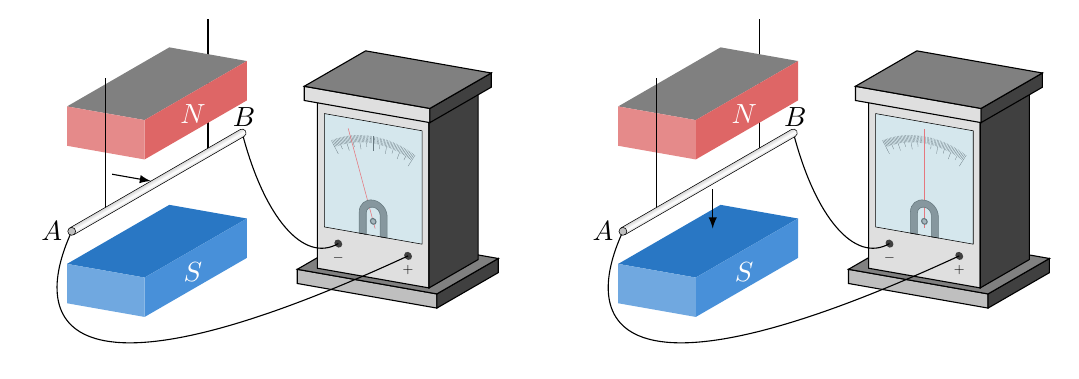
\begin{tikzpicture}[>=latex,scale=1.0]
  \useasboundingbox(-.5,-1.1)rectangle(12.5,3.0);
  \begin{scope}
    \dlj[-16]{xshift=4.2cm}
    \draw(in)..controls(0,-1.9)and(-0.5,-0.8)..(0.0594,0.4132);
    \draw(out)..controls(3,0)and(2.5,0.6)..(2.2245,1.6632);
    \draw(1.79,1.41)--++(0,1.7);
    \fill[azure5](0,0)--(30:1.5)--++(-10:1.0)--++(-150:1.5)--cycle;
    \fill[azure6](-10:1.0)--++(30:1.5)--++(0,-0.5)--++(-150:1.5)--cycle;
    \fill[azure7](0,0)--(-10:1.0)--++(0,-0.5)--++(170:1.0)--cycle;
    \fill[gray](0,2)--++(30:1.5)--++(-10:1.0)--++(-150:1.5)--cycle;
    \fill[red6]([yshift=2cm]-10:1.0)--++(30:1.5)--++(0,-0.5)--++(-150:1.5)--cycle;
    \fill[red7](0,2)--++(-10:1.0)--++(0,-0.5)--++(170:1.0)--cycle;
    \node at (1.6,1.9)[text=white]{$N$};
    \node at (1.6,-0.1)[text=white]{$S$};
    \draw(0.49,0.66)--++(0,1.7);
    \draw[shading=pile,shading angle=30,very thin](0.034,0.456)--(2.199,1.706)arc(120:-60:0.05)node[above]{$B$}--(0.084,0.370)--cycle;
    \draw[fill=lightgray,very thin](0.0594,0.4132)circle(0.05)node[left]{$A$};
    \draw[<-](1.065,1.052)--++(170:0.5);
  \end{scope}
  \begin{scope}[xshift=7cm]
    \dlj[0]{xshift=4.2cm}
    \draw(in)..controls(0,-1.9)and(-0.5,-0.8)..(0.0594,0.4132);
    \draw(out)..controls(3,0)and(2.5,0.6)..(2.2245,1.6632);
    \draw(1.79,1.41)--++(0,1.7);
    \fill[azure5](0,0)--(30:1.5)--++(-10:1.0)--++(-150:1.5)--cycle;
    \fill[azure6](-10:1.0)--++(30:1.5)--++(0,-0.5)--++(-150:1.5)--cycle;
    \fill[azure7](0,0)--(-10:1.0)--++(0,-0.5)--++(170:1.0)--cycle;
    \fill[gray](0,2)--++(30:1.5)--++(-10:1.0)--++(-150:1.5)--cycle;
    \fill[red6]([yshift=2cm]-10:1.0)--++(30:1.5)--++(0,-0.5)--++(-150:1.5)--cycle;
    \fill[red7](0,2)--++(-10:1.0)--++(0,-0.5)--++(170:1.0)--cycle;
    \node at (1.6,1.9)[text=white]{$N$};
    \node at (1.6,-0.1)[text=white]{$S$};
    \draw(0.49,0.66)--++(0,1.7);
    \draw[shading=pile,shading angle=30,very thin](0.034,0.456)--(2.199,1.706)arc(120:-60:0.05)node[above]{$B$}--(0.084,0.370)--cycle;
    \draw[fill=lightgray,very thin](0.0594,0.4132)circle(0.05)node[left]{$A$};
    \draw[->](1.2,0.95)--++(0,-0.5);
  \end{scope}
\end{tikzpicture}
\end{document}